\chapter{Introduction}

I defined \emph{funcoid} and based on this generalized \emph{limit of an arbitrary (even discontinuous) function} in~\cite{volume-1-edition1}.

In this article I consider generalized limits in more details.

This article is written in such a way that a reader could understand the main ideas on generalized limits without resorting to reading~\cite{volume-1-edition1} beforehand, but to follow the proofs you need read that first.

Definition of generalized limit makes it obvious to define such things as derivative of an arbitrary function, integral of an arbitrary function, etc.

Note that generalized limit is a ``composite'' object, not just a simple real number, point, or ``regular'' vector.

\chapter{A popular explanation of generalized limit}

For an example, consider some real function~$f$ from $x$-axis to $y$-axis:
\begin{figure}[H]
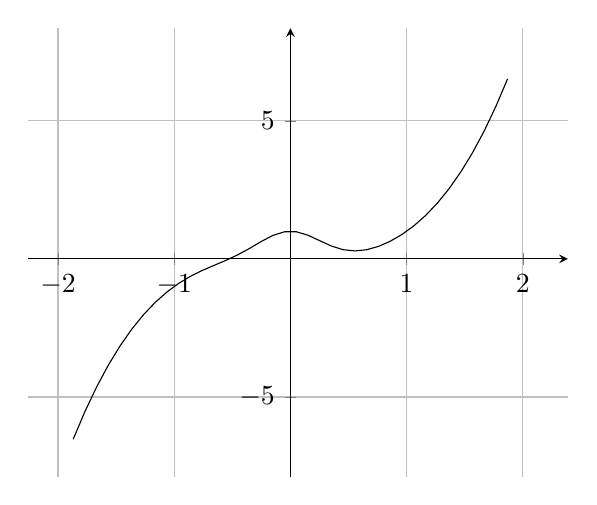
\begin{tikzpicture}
\begin{axis}[grid=both,
          xmax=2,ymax=7,
          axis lines=middle,
          restrict y to domain=-7:7,
          enlargelimits]
\addplot[domain=-5:5,samples=100]{pow(2,-10*x^2)+x^3};
\end{axis}
\end{tikzpicture}
\end{figure}
 
Take it's infinitely small fragment (in our example, an infinitely small interval for~$x$ around zero; see below for an explanation what is infinitely small):
\begin{figure}[H]
\begin{tikzpicture}
\begin{axis}[grid=both,
          xmax=2,ymax=7,
          axis lines=middle,
          restrict y to domain=-7:7,
          enlargelimits]
\addplot[domain=-0.2:0.2,samples=100]{pow(2,-10*x^2)+x^3};
\end{axis}
\end{tikzpicture}
\end{figure}

Next consider that with a value~$y$ replaced with an infinitely small interval like $[y-\epsilon;y+\epsilon]$:
\begin{figure}[H]
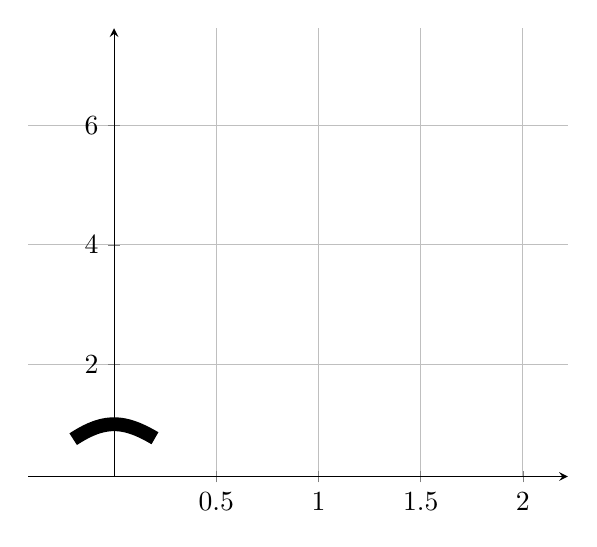
\begin{tikzpicture}
\begin{axis}[grid=both,
          xmax=2,ymax=7,
          axis lines=middle,
          restrict y to domain=-7:7,
          enlargelimits]
\addplot[domain=-0.2:0.2,samples=100,
          line width=5pt]{pow(2,-10*x^2)+x^3};
\end{axis}
\end{tikzpicture}
\end{figure}

Now we have ``an infinitely thin and short strip''. In fact, it is the same as an ``infinitely small rectangle'' (Why? So infinitely small behave, it can be counter-intuitive, but if we consider the above meditations formally, we could get this result):
\begin{figure}[H]
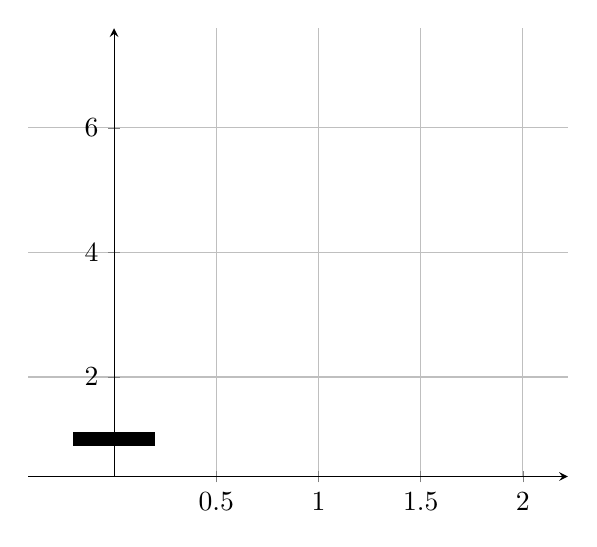
\begin{tikzpicture}
\begin{axis}[grid=both,
          xmax=2,ymax=7,
          axis lines=middle,
          restrict y to domain=-7:7,
          enlargelimits]
\addplot[domain=-0.2:0.2,samples=100,
          line width=5pt]{pow(2,-10)+1};
\end{axis}
\end{tikzpicture}
\end{figure}

This infinitely small rectangle's $y$~position uniquely characterizes the limit of our function (in our example at~$x\to 0$).

If we consider the set of all rectangles we obtain by shifting this rectangle by adding an arbitrary number to~$x$, we get
\begin{figure}[H]
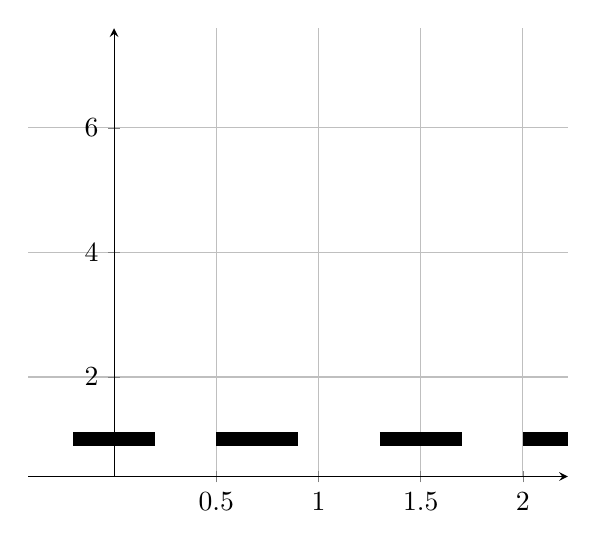
\begin{tikzpicture}
\begin{axis}[grid=both,
          xmax=2,ymax=7,
          axis lines=middle,
          restrict y to domain=-7:7,
          enlargelimits]
\addplot[domain=-0.2:0.2,samples=100,
          line width=5pt]{pow(2,-10)+1};
\addplot[domain=0.5:0.9,samples=100,
          line width=5pt]{pow(2,-10)+1};
\addplot[domain=1.3:1.7,samples=100,
          line width=5pt]{pow(2,-10)+1};
\addplot[domain=2.0:2.4,samples=100,
          line width=5pt]{pow(2,-10)+1};
\addplot[domain=2.7:3.1,samples=100,
          line width=5pt]{pow(2,-10)+1};
\addplot[domain=3.4:3.8,samples=100,
          line width=5pt]{pow(2,-10)+1};
\end{axis}
\end{tikzpicture}
\end{figure}
Such sets one-to-one corresponds to the value of the limit of our function (at $x\to 0$): Knowing such the set, we can calculate the limit (take its arbitrary element and get its so to say $y$-limit point) and knowing the limit value~($y$), we could write down the definition of this set.

So we have a formula for \emph{generalized limit}:
\[ \lim_{x\to a} f(x) =
\{ \mathrm{X} \circ f|_{\Delta(a)} \circ r \mid r\in G \} \]
where~$G$ is the group of all horizontal shifts of our space~$\mathbb{R}$, $f|_{\Delta(a)}$ is the function~$f$ of which we are taking limit restricted to the infinitely small interval~$\Delta(a)$ around the point~$a$, $\mathrm{X}\circ{}$~is ``stretching'' our function graph into the infinitely thin ``strip'' by applying a topological operation to it.

What all this (especially ``infinitely small'') means? It is filters and ``funcoids'' (see below for the definition).

Why we consider all shifts of our infinitely small rectangle? To make the limit not dependent of the point~$a$ to which $x$~tends. Otherwise the limit would depend on the point~$a$.

Note that for discontinuous functions elements of our set (our limit is a set) won't be infinitely small ``rectangles'' (as on the pictures), but would ``touch'' more than just one~$y$ value.

The interesting thing here is that we can apply the above formula to \emph{every} function: for example to a discontinuous function, Dirichlet function, unbounded function, unbounded and discontinuous at every point function, etc. In short, the generalized limit is defined for \emph{every} function. We have a definition of limit for every function, not only a continuous function!

And it works not only for real numbers. It would work for example for any function between two topological vector spaces (a vector space with a topology).

Hurrah! Now we can define derivative and integral of \emph{every} function.

\chapter{Funcoids}

I will reprise (without proofs) several equivalent definitions of funcoid from~\cite{volume-1-edition1}:

Binary relation $\delta$ between two sets (source and destination of the funcoid), conforming to the axioms:

\begin{enumerate}
\item not $\emptyset\mathrel{\delta}X$
\item not $X\mathrel{\delta}\emptyset$
\item $I\cup J \mathrel{\delta} K\iff I \mathrel{\delta}K\wedge J\mathrel{\delta}K$
\item $K\mathrel{\delta}I\cup J\iff K \mathrel{\delta}I\wedge K\mathrel{\delta}J$
\end{enumerate}

Pair of functions $(\alpha,\beta)$ between the sets of filters filters on some two sets (source and destination of the funcoid), conforming to the formula:
\[ \alpha (\mathcal{X})\sqcap \mathcal{Y}\neq \bot \iff \beta (\mathcal{Y})\sqcap \mathcal{X}\neq \bot. \]

\begin{rem}
Funcoid~$(\alpha,\beta)$ is determined by the value of~$\alpha$ (or value of~$\beta$).
\end{rem}

A function $\Delta$ from the set of subsets of some set (source of the funcoid) to the set of filters on some set (destination of the funcoid), conforming to the axioms:

\begin{enumerate}
\item $\Delta (\emptyset)=\bot$
\item $\Delta (X\sqcup Y)=\Delta (X)\sqcup \Delta (Y)$
\end{enumerate}

(Here~$\sqcup$ and~$\sqcap$ are the join and the meet correspondingly on the lattice of filters with order reverse to set-theoretic inclusion, $\bot$~is the improper filter.)

Note that we define things to have the equations:
\begin{enumerate}
\item
\begin{multline*}
X\rsuprel{f}Y \Leftrightarrow X\mathrel{\delta}Y \Leftrightarrow \\ \uparrow X\suprel{(\alpha,\beta)}\uparrow Y \Leftrightarrow
\alpha (X)\sqcap Y\neq \bot \Leftrightarrow \\ \beta (Y)\sqcap X\neq \bot
\end{multline*}
\item $\rsupfun{f}X = \Delta X = \alpha\uparrow X$
\end{enumerate}

We will denote partial orders as~$\sqsubseteq$.

I will call \emph{endofuncoid} a funcoid whose source and destination are the same.

Funcoids form a semigroup (or precategory, dependently on the exact axioms) with the operation defined by the formula:
\[ (\alpha _{1},\beta _{1})\circ (\alpha _{0},\beta _{0})=(\alpha _{1}\circ \alpha _{0},\beta _{0}\circ \beta _{1}). \]

We denote $\supfun{(\alpha,\beta)}=\alpha$ and
$(\alpha,\beta)^{-1} = (\beta,\alpha)$.

Funcoids also form a poset which is a complete lattice.

Funcoids are a generalization of both topological spaces and proximity spaces (see~\cite{volume-1-edition1}).

Also funcoids are~(\cite{volume-1-edition1}) a generalization of binary relations. (I will denote the funcoid corresponding~(\cite{volume-1-edition1}) to a binary relation~$f$ as~$\uparrow f$) This makes funcoids a common generalization for topologies/proximities and functions, so they are a convenient tool to study functions between spaces.

Another important for this article operation on funcoids is \emph{restricting} a funcoid to a filter (generalizing restricting a function to a set):~$f|_{\mathcal{X}}$ for a funcoid~$f$ and filter~$\mathcal{X}$.

In~\cite{volume-1-edition1} we also have a funcoid called \emph{funcoidal product} $\mathcal{X}\times^{\mathsf{FCD}}\mathcal{Y}$ of two filters~$\mathcal{X}$ and~$\mathcal{Y}$.

\chapter{Limit for funcoids}

The following is a straigthforward generalization of the well known concepts of adherent point of a set (more generally a cluster point of a filter), a limit point of a filter, a and limit of a function in a
topological space.

\begin{note}
Due to an unfortunate choice of terminology, limit point of a filter is \emph{not} a generalization of a limit point of a set.
Limit point for a set isn't a beautiful term and we won't use it (in this work), so by \emph{limit point} we will always mean a limit point of a filter.
\end{note}

So, generalizing the corresponding concepts for topological spaces:

Let $d$ be a funcoid.

\begin{defn}
The set of \emph{adherent points} of~$\mathcal{A}$ is
$\Cor\supfun{d^{-1}}\mathcal{A}$ or what is the same
$\setcond{x}{\supfun{d}\{x\}\nasymp\mathcal{A}}$.
\end{defn}

\begin{prop}
There exists a (unique) funcoid $\mathrm{A}$ such that
$\supfun{\mathrm{A}}\mathcal{A}$ is exactly the set of adherent points of~$\mathcal{A}$.
\end{prop}

\begin{proof}
Prove it directly or using that $\Cor$ is a component of a funcoid.
\end{proof}

\begin{defn}
\emph{Limit point} of a filter~$\mathcal{A}$ on $\Dst\mathrm{X}$ is
an~$x\in\Dst\mathcal{A}$ such that
$\rsupfun{d}\{x\}\sqsupseteq\mathcal{A}$.
\end{defn}

\begin{prop}
If $d$ is reflexive, then
there exists a (unique) ``dual funcoid'' (a pointfree funcoid) $\mathrm{L}: \Ob d\to(\Ob d)^{\dual}$ such that
$\supfun{\mathrm{L}}\mathcal{A}$ is exactly the set of limit points of~$\mathcal{A}$.
\end{prop}

\begin{proof}
The set of limit points of the empty set is the maximal set.

The set of limit points of $A\cup B$ (for sets~$A$,~$B$) is the
set of points~$x$ such that $\supfun{d}\{x\}\sqsupseteq A\cup B$ that is $\supfun{d}\{x\}\sqsupseteq A$ and $\supfun{d}\{x\}\sqsupseteq B$ that is the intersection of
the set of limit points of~$A$ and~$B$.

Thus the set of limit points is a component of such a pointfree funcoid.
\end{proof}

\begin{prop}
$\mathrm{L}$ and~$\mathrm{A}$ coincide on ultrafilters.
\end{prop}

\begin{proof}
Because $\rsupfun{d}\{x\}\nasymp a\Leftrightarrow\rsupfun{d}\{x\}\sqsupseteq a$ for an ultrafilter~$a$.
\end{proof}

We have shown that concepts of both limit points and adherent points are essentially funcoids. In traditional general topology limit of a function is defined using limit points of a filter. We will generalize it to limit regarding an arbitrary funcoid (in place of the funcoid describing limit points). We will call this
arbitrary funcoid \emph{the point funcoid} and denote it~$\mathrm{X}$.

\begin{defn}
\emph{Limit} of a funcoid~$f$ is
the filter \[ \lim f=\im(\mathrm{X}\circ f). \]
\end{defn}

\begin{defn}
\emph{Limit} of a funcoid~$f$ at a filter~$\mathcal{X}$ is
the filter \[ \lim_{\mathcal{X}}f=\lim f|_{\mathcal{X}}=\supfun{\mathrm{X}\circ f}\mathcal{X}. \]
\end{defn}

\begin{rem}
If $\mathrm{X}=\mathrm{L}$, then the limit is either an one-element or an empty set (``no limit'' in traditional topology).
\end{rem}

In~\cite{volume-1-edition1} limit for a funcoid~$f$ was defined this way: $f$~\emph{tends} to filter~$\mathcal{A}$ ($f\to \mathcal{A}$) regarding a funcoid~$\mathrm{X}$ on a filter~$\mathcal{X}$ iff
\[ \im f \sqsubseteq \supfun{\mathrm{X}}\mathcal{A}. \]

$\lim f$ is such a point that $f$~tends to $\lim f$.

\begin{prop}
That definition from~\cite{volume-1-edition1} coincides with
our above definition, if $\mathrm{X}=\mathrm{L}$.
\end{prop}

\begin{proof}
In this proof $\lim f$ will mean our definition, \emph{not} the definition from~\cite{volume-1-edition1}. We need to prove that
$\lim f=\setcond{x}{\im f\sqsubseteq\rsupfun{\mathrm{X}}\{x\}}$.

Really,
\[
\lim f=\im(\mathrm{L}\circ f) = 
\supfun{\mathrm{L}}\im f =
\setcond{x}{\rsupfun{\mathrm{X}}\{x\}\sqsupseteq\im f}.
\]
\end{proof}

If $\mathrm{X}$~is Hausdorff ($T_2$-separable) (see~\cite{volume-1-edition1}), then there exists no more than one~$\lim f$.

\chapter{Axiomatic generalized limit}

Let~$\mathrm{X}$ be a (fixed) funcoid. For example, $\mathrm{X}=d$ where $d$~is
some proximity or $d=\mathrm{A}$ or $d=\mathrm{L}$ (up to a duality).

By definion $\lim_{\mathcal{X}}f = \supfun{\mathrm{X}\circ f}\mathcal{X}$ (for every funcoid~$f$).

\begin{rem}
If $\supfun{\mathrm{X}}y$ is an limit point (considered as an one-element set) of~$y$ and $f$~is a function, then the above
defined~$\lim$ is the
same as limit in traditional calculus and topology (except
that it is an one-element set of points instead of a point).
Empty set means ``no limit''.
\end{rem}

Let some group~$G$ (e.g. the group of all shifts on a vector
space, to give an example) is fixed.

\begin{defn}
\emph{Axiomatic generalized limit} is a two-arguments function $(f,\mathcal{X})\mapsto\xlim_{\mathcal{X}}f$
from the set $\funcoids(A,B)\times\mathscr{F}(A)$ to the set of functions defined on filters~$\mathcal{C}$ such that exists $r\in G$ such that $\mathcal{C}\sqsubseteq\supfun{r}\mathcal{X}$ by the formula:
\[
(\xlim_{\mathcal{X}}f)\mathcal{C} = \lim_{\supfun{r^{-1}}\mathcal{C}} f.
\]
\end{defn}

\begin{rem}
Its meaning is that $\lim_{\mathcal{C}} f$ can be restored from
$\xlim_{\mathcal{X}}f$.
\end{rem}

\begin{prop}
To describe an axiomatic generalized limit, it's enough to define
it on ultrafilters.
\end{prop}

\begin{proof}
Easily follows from the fact that a funcoid is described by its values on ultrafilters.
\end{proof}

Thus axiomatic generalized limit gives a detailed behavior of
a function at a filter (its limit at every its atomic subfilter).

\begin{obvious}
$\xlim_{\mathcal{X}}f = \xlim_{\supfun{r}\mathcal{X}}(f\circ r^{-1})$ for every~$r\in G$.
\end{obvious}

\begin{thm}
$\lim_{\mathcal{X}} f$ can be restored knowing $\xlim_{\mathcal{X}} f$.
\end{thm}

\begin{proof}
\begin{multline*}
\lim_{\mathcal{X}} f = \supfun{\mathrm{X}\circ f}\mathcal{X} =
\bigsqcup_{x\in\atoms\mathcal{X}} \supfun{\mathrm{X}\circ f}x = \\
\bigsqcup_{x\in\atoms\mathcal{X}} \lim x =
(\xlim_{\mathcal{X}}f)x.
\end{multline*}
\end{proof}

Let~$y$ be an arbitrary point of the space~$\Dst\mathrm{X}$. Consider
the constant function~$f$ whose value is this~$y$.
Then the first axiom above determines the $\xlim_{\mathcal{C}} f$
for every filter~$\mathcal{C}$.

I will denote $\xlim_{\mathcal{C}} f = \tau(y)$.

\begin{rem}
The above easily generalizes for~$y$ being a set of points.
\end{rem}

\begin{obvious}
$\tau$~is an injection, if $\Src\mathrm{X}$ is a non-empty set and
$\supfun{\mathrm{X}}$~is an injection on one-element sets.
\end{obvious}

\begin{cor}
$\tau$~is an injection, if $\Src\mathrm{X}$ is a non-empty set and
$\mathrm{X}=\mathrm{A}$ and $\mathrm{X}$~is Hausdorff.
\end{cor}

In other words, on Hausdorff topologies the set of singularities
with non-empty domains is an extension of the set of points~$\Dst\mathrm{X}$ (up to a bijection).

\chapter{Generalized limit}

\section{The definition of generalized limit}

In~\cite{volume-1-edition1} generalized limit is defined like the formula:

\begin{equation}\label{xlim1}
\xlim f = \setcond{ \mathrm{X}\circ f\circ \uparrow r}{r\in G}.
\end{equation}

We suppose:

Let $\mu$ and $\mathrm{X}$ be endofuncoids (on sets~$\Ob\mu$,~$\Ob\mathrm{X}$). Let $G$ be a transitive permutation
group on $\Ob\mu$.

We require that $\mu$ and every $r\in G$ commute, that is
\begin{equation}\label{commute}
\mu\circ\uparrow r=\uparrow r\circ\mu.
\end{equation}

We require for every $y\in\Ob\mathrm{X}$ 
\begin{equation}\label{lim-squares}
\mathrm{X}\sqsupseteq\supfun{\mathrm{X}}\uparrow\{y\}\times^{\mathsf{FCD}}\supfun{\mathrm{X}}\uparrow\{y\}.
\end{equation}

\begin{prop}
Formula (\ref{lim-squares}) follows from $\mathrm{X}\sqsupseteq\mathrm{X}\circ\mathrm{X}^{-1}$.
\end{prop}

\begin{proof}
Let $\mathrm{X}\sqsupseteq\mathrm{X}\circ\mathrm{X}^{-1}$. Then
\begin{align*}
\supfun{\mathrm{X}}\uparrow\{y\}\times^{\mathsf{FCD}}\supfun{\mathrm{X}}\uparrow\{y\} & =\\
\mathrm{X}\circ(\uparrow\{y\}\times^{\mathsf{FCD}}\uparrow\{y\})\circ\mathrm{X}^{-1} & =\\
\mathrm{X}\circ\uparrow(\{y\}\times\{y\})\circ\mathrm{X}^{-1} & \sqsubseteq\\
\mathrm{X}\circ 1\circ\mathrm{X}^{-1} & =\\
\mathrm{X}\circ\mathrm{X}^{-1} & \sqsubseteq\mathrm{X}.
\end{align*}
(Here~$1$ is the identity element of the semigroup of endofuncoids.)
\end{proof}

So we have (generalized) limits of arbitrary functions
acting from $\Ob\mu$ to $\Ob\mathrm{X}$. (The functions in consideration
are not required to be continuous.)

\begin{rem}
Most typically $G$ is the group of translations of some topological vector space\footnote{I remind that every Banach space, every normed space, and every Hilbert space is a vector topological space.}. So in particular we have defined limit of an arbitrary function acting from a vector topological space to a topological space.
\end{rem}

\section[Injection to generalized limits]{Injection from the set of points to the set of all generalized limits}

The function $\tau$ will define an injection from the set of points
of the space $\mathrm{X}$ (``numbers'', ``points'', or ``vectors'')
to the set of all (generalized) limits (i.e. values which $\xlim_{x}f$
may take).
\begin{defn}
\[ \tau(y)\eqdef\setcond{\supfun{\mu}\uparrow\{x\}\times^{\mathsf{FCD}}\supfun{\mathrm{X}}\uparrow\{y\}}{x\in D}. \]
\end{defn}
\begin{prop}
\[ \tau(y)=\setcond{(\supfun{\mu}\uparrow\{x\}\times^{\mathsf{FCD}}\supfun{\mathrm{X}}\uparrow\{y\})\circ\uparrow r}{r\in G} \]
for every (fixed) $x\in D$.\end{prop}

\begin{proof}
~
\begin{align*}
(\supfun{\mu}\uparrow\{x\}\times^{\mathsf{FCD}}\supfun{\mathrm{X}}\uparrow\{y\})\circ\uparrow r & =\\
\supfun{\uparrow r^{-1}}\supfun{\mu}\uparrow\{x\}\times^{\mathsf{FCD}}\supfun{\mathrm{X}}\uparrow\{y\} & =\\
\supfun{\mu}\supfun{\uparrow r^{-1}}\uparrow\{x\}\times^{\mathsf{FCD}}\supfun{\mathrm{X}}\uparrow\{y\} & =\\
\supfun{\mu}\uparrow\{r^{-1}x\}\times^{\mathsf{FCD}}\supfun{\mathrm{X}}\uparrow\{y\} & \in \\ \setcond{\supfun{\mu}\uparrow\{x\}\times^{\mathsf{FCD}}\supfun{\mathrm{X}}\uparrow\{y\}}{x\in D}.
\end{align*}


Reversely
\begin{multline*}
\supfun{\mu}\uparrow\{x\}\times^{\mathsf{FCD}}\supfun{\mathrm{X}}\uparrow\{y\}=\\(\supfun{\mu}\uparrow\{x\}\times^{\mathsf{FCD}}\supfun{\mathrm{X}}\uparrow\{y\})\circ\uparrow e
\end{multline*}
where $e$ is the identify element of $G$.\end{proof}

\begin{prop}
\[ \tau(y)=\xlim(\supfun{\mu}\uparrow\{x\}\times^{\mathsf{FCD}}\uparrow\{y\}) \]
(for every $x$). Informally: Every $\tau(y)$ is a generalized limit
of a constant function.
\end{prop}

\begin{proof}
~
\begin{align*}
\xlim(\supfun{\mu}\uparrow\{x\}\times^{\mathsf{FCD}}\uparrow\{y\}) & =\\
\setcond{\mathrm{X}\circ(\supfun{\mu}\uparrow\{x\}\times^{\mathsf{FCD}}\uparrow\{y\})\circ\uparrow r}{r\in G} & =\\
\setcond{(\supfun{\mu}\uparrow\{x\}\times^{\mathsf{FCD}}\supfun{\mathrm{X}}\uparrow\{y\})\circ\uparrow r}{r\in G} & =\tau(y).
\end{align*}
\end{proof}

\begin{cor}
The~$\tau$ defined in this section for generalized limits ``coincides'' with the~$\tau$ defined in the section about axiomatic generalized limits.
\end{cor}

In further we will use on of the definitions of continuity from~\cite{volume-1-edition1}:
\[ f\in\continuous(\mu,\mathrm{X})\Leftrightarrow
f\circ\mu \sqsubseteq \mathrm{X}\circ f \]
and other notation from the book.

\begin{thm}
If $f$ is a function and $f|_{\supfun{\mu}\uparrow\{x\}}\in\continuous(\mu,\mathrm{X})$
and $\supfun{\mu}\uparrow\{x\}\sqsupseteq\uparrow\{x\}$
then $\xlim_{x}f=\tau(fx)$.\end{thm}

\begin{proof}
$f|_{\supfun{\mu}\uparrow\{x\}}\circ\mu\sqsubseteq\mathrm{X}\circ f|_{\supfun{\mu}\uparrow\{x\}}\sqsubseteq\mathrm{X}\circ f$;
thus $\langle f\rangle\supfun{\mu}\uparrow\{x\}\sqsubseteq\supfun{\mathrm{X}}\supfun{f}\uparrow\{x\}$;
consequently we have
\begin{gather*}
\mathrm{X}\sqsupseteq\supfun{\mathrm{X}}\supfun{f}\uparrow\{x\}\times^{\mathsf{FCD}}\supfun{\mathrm{X}}\supfun{f}\uparrow\{x\}\sqsupseteq\\\supfun f\supfun{\mu}\uparrow\{x\}\times^{\mathsf{FCD}}\supfun{\mathrm{X}}\supfun{f}\uparrow\{x\}.\\
\begin{aligned}\mathrm{X}\circ f|_{\supfun{\mu}\uparrow\{x\}} & \sqsupseteq\\
(\supfun f\supfun{\mu}\uparrow\{x\}\times^{\mathsf{FCD}}\supfun{\mathrm{X}}\supfun{f}\uparrow\{x\})\circ f|_{\supfun{\mu}\uparrow\{x\}} & =\\
(f|_{\supfun{\mu}\uparrow\{x\}})^{-1}\supfun f\supfun{\mu}\uparrow\{x\}\times^{\mathsf{FCD}}\supfun{\mathrm{X}}\supfun{f}\uparrow\{x\} & \sqsupseteq\\
\supfun{\id_{\dom f|_{\supfun{\mu}\uparrow\{x\}}}^{\mathsf{FCD}}}\supfun{\mu}\uparrow\{x\}\times^{\mathsf{FCD}}\supfun{\mathrm{X}}\supfun{f}\uparrow\{x\} & \sqsupseteq\\
\dom f|_{\supfun{\mu}\uparrow\{x\}}\times^{\mathsf{FCD}}\supfun{\mathrm{X}}\supfun{f}\uparrow\{x\} & =\\
\supfun{\mu}\uparrow\{x\}\times^{\mathsf{FCD}}\supfun{\mathrm{X}}\supfun{f}\uparrow\{x\}.
\end{aligned}
\end{gather*}


$\im(\mathrm{X}\circ f|_{\supfun{\mu}\uparrow\{x\}})=\supfun{\mathrm{X}}\supfun{f}\uparrow\{x\}$;
\begin{align*}
\mathrm{X}\circ f|_{\supfun{\mu}\uparrow\{x\}} & \sqsubseteq\\
\supfun{\mu}\uparrow\{x\}\times^{\mathsf{FCD}}\im(\mathrm{X}\circ f|_{\supfun{\mu}\uparrow\{x\}}) & =\\
\supfun{\mu}\uparrow\{x\}\times^{\mathsf{FCD}}\supfun{\mathrm{X}}\supfun{f}\uparrow\{x\}.
\end{align*}
So $\mathrm{X}\circ f|_{\supfun{\mu}\uparrow\{x\}}=\supfun{\mu}\uparrow\{x\}\times^{\mathsf{FCD}}\supfun{\mathrm{X}}\supfun{f}\uparrow\{x\}$.

Thus
\begin{multline*}
\xlim_{x}f= \\ \setcond{(\supfun{\mu}\uparrow\{x\}\times^{\mathsf{FCD}}\supfun{\mathrm{X}}\supfun{f}\uparrow\{x\})\circ\uparrow r}{r\in G}= \\ \tau(fx).
\end{multline*}
\end{proof}
\begin{rem}
Without the requirement of $\supfun{\mu}\uparrow\{x\}\sqsupseteq\uparrow\{x\}$
the last theorem would not work in the case of removable singularity.\end{rem}
\begin{thm}
Let $\mathrm{X}\sqsubseteq\mathrm{X}\circ\mathrm{X}$. If $f|_{\supfun{\mu}\uparrow\{x\}}\overset{\mathrm{X}}{\rightarrow}\uparrow\{y\}$
then $\xlim_{x}f=\tau(y)$.\end{thm}

\begin{proof}
$\im f|_{\supfun{\mu}\uparrow\{x\}}\sqsubseteq\supfun{\mathrm{X}}\uparrow\{y\}$;
$\supfun f\supfun{\mu}\uparrow\{x\}\sqsubseteq\supfun{\mathrm{X}}\uparrow\{y\}$;
\begin{align*}
\mathrm{X}\circ f|_{\supfun{\mu}\uparrow\{x\}} & \sqsupseteq\\
(\supfun{\mathrm{X}}\uparrow\{y\}\times^{\mathsf{FCD}}\supfun{\mathrm{X}}\uparrow\{y\})\circ f|_{\supfun{\mu}\uparrow\{x\}} & =\\
\supfun{(f|_{\supfun{\mu}\uparrow\{x\}})^{-1}}\supfun{\mathrm{X}}\uparrow\{y\}\times^{\mathsf{FCD}}\supfun{\mathrm{X}}\uparrow\{y\} & =\\
\supfun{\id_{\supfun{\mu}\uparrow\{x\}}^{\mathsf{FCD}}\circ f^{-1}}\supfun{\mathrm{X}}\uparrow\{y\}\times^{\mathsf{FCD}}\supfun{\mathrm{X}}\uparrow\{y\} & \sqsupseteq\\
\supfun{\id_{\supfun{\mu}\uparrow\{x\}}^{\mathsf{FCD}}\circ f^{-1}}\supfun f\supfun{\mu}\uparrow\{x\}\times^{\mathsf{FCD}}\supfun{\mathrm{X}}\uparrow\{y\} & =\\
\supfun{\id_{\supfun{\mu}\uparrow\{x\}}^{\mathsf{FCD}}}\supfun{f^{-1}\circ f}\supfun{\mu}\uparrow\{x\}\times^{\mathsf{FCD}}\supfun{\mathrm{X}}\uparrow\{y\} & \sqsupseteq\\
\supfun{\id_{\supfun{\mu}\uparrow\{x\}}^{\mathsf{FCD}}}\supfun{\id_{\supfun{\mu}\uparrow\{x\}}^{\mathsf{FCD}}}\supfun{\mu}\uparrow\{x\}\times^{\mathsf{FCD}}\supfun{\mathrm{X}}\uparrow\{y\} & =\\
\supfun{\mu}\uparrow\{x\}\times^{\mathsf{FCD}}\supfun{\mathrm{X}}\uparrow\{y\}.
\end{align*}

On the other hand, \[ f|_{\supfun{\mu}\uparrow\{x\}}\sqsubseteq\supfun{\mu}\uparrow\{x\}\times^{\mathsf{FCD}}\supfun{\mathrm{X}}\uparrow\{y\}; \]

\begin{multline*}
\mathrm{X}\circ f|_{\supfun{\mu}\uparrow\{x\}}\sqsubseteq\supfun{\mu}\uparrow\{x\}\times^{\mathsf{FCD}}\supfun{\mathrm{X}}\supfun{\mathrm{X}}\uparrow\{y\}\sqsubseteq\\\supfun{\mu}\uparrow\{x\}\times^{\mathsf{FCD}}\supfun{\mathrm{X}}\uparrow\{y\}.
\end{multline*}

So $\mathrm{X}\circ f|_{\supfun{\mu}\uparrow\{x\}}=\supfun{\mu}\uparrow\{x\}\times^{\mathsf{FCD}}\supfun{\mathrm{X}}\uparrow\{y\}$.

\begin{multline*}
\xlim_{x}f=\setcond{\mathrm{X}\circ f|_{\supfun{\mu}\uparrow\{x\}}\circ\uparrow r}{r\in G}=\\ \setcond{(\supfun{\mu}\uparrow\{x\}\times^{\mathsf{FCD}}\supfun{\mathrm{X}}\uparrow\{y\})\circ\uparrow r}{r\in G}=\tau(y).
\end{multline*}
\end{proof}
\begin{cor}
If $\lim_{\supfun{\mu}\uparrow\{x\}}^{\mathrm{X}}f=y$ then $\xlim_{x}f=\tau(y)$ (provided that $\mathrm{X}\sqsubseteq\mathrm{X}\circ\mathrm{X}$).
\end{cor}
We have injective $\tau$ if $\supfun{\mathrm{X}}\uparrow\{y_{1}\}\sqcap\supfun{\mathrm{X}}\uparrow\{y_{2}\}=\bot^{\mathscr{F}(\Ob\mu)}$
for every distinct $y_{1},y_{2}\in\Ob\mathrm{X}$ that is if $\mathrm{X}$ is $T_{2}$-separable.

\section{Hausdorff and Kolmogorov funcoids}

\begin{defn}
A funcoid~$f$ is \emph{Kolmogorov} when
$\supfun{f}\uparrow\{x\}\ne\supfun{f}\uparrow\{y\}$ for every distinct points
$x,y\in\dom f$.
\end{defn}

\begin{defn}
\emph{Limit}~$\lim\mathcal{F}=x$ of a filter~$\mathcal{F}$
regarding funcoid~$f$ is such a point that $\supfun{f}\uparrow\{x\}\sqsupseteq\mathcal{F}$.
\end{defn}

\begin{defn}
\emph{Hausdorff} funcoid is such a funcoid that every proper
filter on its image has at most one limit.
\end{defn}

\begin{prop}
The following are pairwise equivalent for every funcoid~$f$:
\begin{enumerate}
\item\label{hd:eq-d} $f$~is Hausdorff.
\item\label{hd:eq-op}
$x\ne y\Rightarrow\supfun{f}\uparrow\{x\}\sqcap\supfun{f}\uparrow\{y\}=\bot$.
\end{enumerate}
\end{prop}

\begin{proof}
~
\begin{description}
\item[\ref{hd:eq-d}$\Rightarrow$\ref{hd:eq-op}]
If~\ref{hd:eq-op} does not hold,
then there exist distinct points~$x$ and~$y$ such that
$\supfun{f}\uparrow\{x\}\sqcap\supfun{f}\uparrow\{y\}\ne\bot$.
So~$x$ and~$y$ are both limit points of
$\supfun{f}\uparrow\{x\}\sqcap\supfun{f}\uparrow\{y\}$, and thus~$f$ is not
Hausdorff.
\item[\ref{hd:eq-op}$\Rightarrow$\ref{hd:eq-d}]
Suppose~$\mathcal{F}$ is proper.
\begin{multline*}
\supfun{f}\uparrow\{x\}\sqsupseteq\mathcal{F}\land
\supfun{f}\uparrow\{y\}\sqsupseteq\mathcal{F}\Rightarrow \\
\supfun{f}\uparrow\{x\}\sqcap\supfun{f}\uparrow\{y\}\ne\bot \Rightarrow x=y.
\end{multline*}
\end{description}
\end{proof}

\begin{cor}
Every entirely defined Hausdorff funcoid is Kolmogorov.
\end{cor}

\begin{rem}
It is enough to be ``almost entirely defined'' (having nonempty
value everywhere except of one point).
\end{rem}

\begin{obvious}
For a complete funcoid induced by a topological space this
coincides with the traditional definition of a Hausdorff
topological space.
\end{obvious}

\chapter{Generalized limit vs axiomatic generalized limit}

I will call \emph{singularities} the set of generalized limits of the form $\xlim_{\supfun{\mu}\uparrow\{x\}}f$ where $f$~is an entirely defined funcoid and $x$~ranges all points of~$\Ob\mu$.

I will call \emph{axiomatic singularities} the set of axiomatic generalized limits of the form $\xlim_{\supfun{\mu}\uparrow\{x\}}f$ where $f$~is an entirely defined funcoid and $x$~ranges all points of~$\Ob\mu$.

Switching back and forth between generalized limits and what I call $F$-singularities:
\begin{gather*}
\Phi f =\setcond{(\dom F, F)}{F \in f};\\
\Psi f = \im f.
\end{gather*}

\begin{prop}
Let the funcoid~$\mu$ is Kolmogorov and~$\mathrm{X}$ is entirely defined. Then $\Phi$ is an injection from the set of singularities to the set of monovalued functions.
\end{prop}

\begin{proof}
That it's an injection is obvious.

We need to prove that $\dom F_0\ne\dom F_1$ for each~$F_0,F_1\in f$ such that $F_0\ne F_1$.
Really, $F_0=\mathrm{X}\circ f|_{\supfun{\mu}\uparrow\{x_0\}}\circ\uparrow r_0$ for $x_0\in\Ob\mu$, $r_0\in G$.
We have $\dom F_0 = \dom f|_{\supfun{\mu}\uparrow\{x_0\}}=\supfun{\mu}\uparrow\{x_0\}$. Similarly $\dom F_1=\supfun{\mu}\uparrow\{x_1\}$ for some $x_1\in\Ob\mu$.
Thus $\dom F_0\ne\dom F_1$ because otherwise $x_0=x_1$ and so $r_0\ne r_1$,
\begin{multline*}
\dom F_0=\supfun{\uparrow r_0^{-1}}\supfun{\mu}\uparrow\{x_0\}=\\\supfun{\mu}\supfun{\uparrow r_0^{-1}}\uparrow\{x_0\}\ne\\\text{(Kolmogorov property)}\ne\\\supfun{\mu}\supfun{\uparrow r_1^{-1}}\{x_0\}=\\\supfun{\uparrow r_1^{-1}}\supfun{\mu}\{x_0\}=\dom F_1,
\end{multline*}
contradiction.

It remains to prove that $(f,\mathcal{X})\mapsto\Phi(\xlim_{\mathcal{X}} f)$ conforms to the axioms.

The second axiom is obvious.

It remains to prove that
\[ \supfun{\Phi(\xlim_{\mathcal{X}} f)}\mathcal{C} = \lim_{\mathcal{C}}f. \]
Really, $\Phi(\xlim_{\mathcal{X}} f)$ is equal to an $F\in\xlim_{\mathcal{X}} f$ such that $\dom F=\mathcal{X}$.
So $F=\mathrm{X}\circ f$.
\[ \supfun{\Phi(\xlim_{\mathcal{X}} f)}\mathcal{C} =
\supfun{\mathrm{X}\circ f}\mathcal{C} =
\supfun{\mathrm{X}\circ f}\mathcal{C} =
\lim_{\mathcal{C}}f. \]
\end{proof}

\begin{thm}
The following are mutually inverse bijections between
generalized limits and axiomatic generalized limits on a filter~$\mathcal{X}$ such that $\supfun{r}\mathcal{X}\asymp\mathcal{X}$ for all $r\in G\setminus\{e\}$:
\begin{enumerate}
\item\label{corr-gl-agl} Let~$y$ be a generalized limit. The corresponding axiomatic
generalized limit maps~$\mathcal{C}$ to $\supfun{f}\mathcal{C}$ whenever $f\in y$ and $\mathcal{C}\sqsubseteq\dom f$ and is undefined if there is no such~$f$. (Remark: obviously $y\ne\emptyset$.)
\item\label{corr-agl-gl} Let~$u$ be an axiomatic generalized limit. The corresponding generalized limit~$y$ is a set of funcoids (of suitable source and destination) such that
\[q\in y \Leftrightarrow \supfun{q}\mathcal{C}=\begin{cases}
u\mathcal{C}&\text{if }\mathcal{C}\in\dom u;\\
\emptyset&\text{otherwise}.
\end{cases}
\]
\end{enumerate}
\end{thm}

\begin{proof}
First, we need to prove that the mapping from~$\mathcal{C}$ to~$\supfun{f}\mathcal{C}$ is monovalued. For $\mathcal{C}=\emptyset$ it's obvious. It's enough to show that $f_0=f_1$ if $f_0,f_1\in y$ and $\mathcal{C}\sqsubseteq\dom f_0\land\mathcal{C}\sqsubseteq\dom f_1$. But for $\mathcal{C}\ne\emptyset$ it follows from the fact that $\dom f_0\asymp\dom f_1$ for $f_0\ne f_1$ as directly follow from theorem conditions.

Next we need to show that our functions are mutually inverse.

Let~$y_0$ be a generalized limit. Let~$u$ be the axiomatic generalized limit corresponding to it by~\ref{corr-gl-agl}. Let $y_1$ be the generalized limit corresponding to it by~\ref{corr-agl-gl}. Then
\[q\in y_1 \Leftrightarrow \forall\mathcal{C}:\supfun{q}\mathcal{C}=\begin{cases}
\supfun{f}\mathcal{C}&\text{if }\mathcal{C}\sqsubseteq\dom f;\\
\emptyset&\text{otherwise};
\end{cases} \Leftrightarrow q=f
\]
for some $f\in y_0$. That is, if $q\in y_1$ then $q=f$ for some $f\in y_0$ and if $q=f$ for some $f\in y_0$ then $f\in y_1$. So $y_0=y_1$.

Let now $u_0$ be an axiomatic generalized limit. Let~$y$ be the generalized limit corresponding to it by by~\ref{corr-agl-gl}. Let $u_1$ be the axiomatic generalized limit corresponding to it by~\ref{corr-gl-agl}. Then~$u_1$ maps~$\mathcal{C}$ to $\supfun{f}\mathcal{C}$ whenever $f\in y$ that is whenever
\[\supfun{f}\mathcal{C}=\begin{cases}
u_0\mathcal{C}&\text{if }\mathcal{C}\in\dom u_0;\\
\emptyset&\text{otherwise}.
\end{cases}
\] and $\mathcal{C}\sqsubseteq\dom f$ and it undefined if there is no such~$f$.
In other words, $u_1$ maps~$\mathcal{C}$ to $u_0\mathcal{C}$ if~$\mathcal{C}\in\dom u_0$ (the case ``otherwise'' is not to be considered because $\dom u_1=\dom u_0$). So $u_1=u_0$.
\end{proof}

So if we define a function on the set of functions whose values are funcoids, we automatically define (as this injection preimage) a function on the set of singularities. Let's do it.

Let $\varphi$ be a (possibly multivalued) multiargument function.

\chapter{Operations on generalized limits}

\section{Applying functions to functions}

As usually in calculus:

Let~$\varphi$ is an arbitrary multiargument function.

\begin{defn}
$(\varphi f) x = \varphi (\lambda i \in D : f_i x)$
for an indexed (by $\dom\varphi$) family $f$ of functions of the same domain $D$ to domains of arguments of~$\varphi$.
\end{defn}

\section{Applying functions to sets}

\begin{defn}
  $\varphi X = \rsupfun{\varphi} \prod X$ for a family $X$ of sets, where each $X_i$ is an element of the domain of $i$-th element of~$\varphi$.
\end{defn}

\begin{obvious}
$\varphi (\lambda i \in D : \{ x_0 \}) = \{ \varphi x \}$.
\end{obvious}

\section{Applying functions to filters}

\begin{defn}
  $\varphi x = \supfun{\varphi} \prod^{\reloids}_{X \in \prod x} X$ for a
  family $x$ of atomic filters.
\end{defn}

\begin{prop}
  $\varphi$ can be continued to a pointfree funcoid.
\end{prop}

\begin{proof}
  Need to prove (theorem 1650 in~\cite{volume-1-edition1})
  \[ \supfun{\varphi} \prod^{\reloids}_{X \in \prod a} X \sqsubseteq \bigsqcap
     \setcond{\bigsqcup \rsupfun{x \mapsto \supfun{\varphi}
     \prod^{\reloids}_{X \in \prod x} X} \atoms \mathcal{X}}{\mathcal{X} \in
     \up a} . \]
  Really,
\begin{multline*}
\bigsqcup \rsupfun{x \mapsto \supfun{\varphi} \prod^{\reloids}_{X \in
     \prod x} X} \atoms \mathcal{X} =\\ \supfun{\varphi} \bigsqcup \rsupfun{x
     \mapsto \prod^{\reloids}_{X \in \prod x} X} \atoms \mathcal{X} .
\end{multline*}
  But by theorem 1875 in~\cite{volume-1-edition1}:
  \[ \bigsqcup \rsupfun{x \mapsto \prod^{\reloids}_{X \in \prod x} X}
     \atoms \mathcal{X} = \prod^{\reloids}_{X \in \prod \mathcal{X}}
     X . \]
  So, $\bigsqcup \rsupfun{x \mapsto \prod^{\reloids}_{X \in \prod a} X}
  \atoms \mathcal{X} \sqsupseteq \prod^{\reloids}_{X \in \prod a}
  \mathcal{X}$. Thus follows the thesis.
\end{proof}

\section{Applying functions to funcoids}

\begin{defn}
For a family $f$ of funcoids having a common source set and filter on this set
  $\mathcal{X}$
\[(\varphi f) \mathcal{X} = \varphi \left( \lambda i \in \dom f :
  \supfun{f_i} \mathcal{X} \right) .\]
\end{defn}

\begin{prop}
  It is a component of a funcoid.
\end{prop}

\begin{proof}
  As composition of two components of pointfree funcoids:
  
  $\varphi (f_0, \ldots, f_n) = \varphi \circ \left( \mathcal{X} \mapsto
  \left( \lambda i \in \dom f : \supfun{f_i} \mathcal{X} \right)
  \right)$.
  
  Note that $\mathcal{X} \mapsto \left( \lambda i \in \dom f :
  \supfun{f_i} \mathcal{X} \right)$ is a component of a pointfree funcoid because
  
\begin{multline*}
  \mathcal{Y} \nasymp \left( \lambda i \in \dom f : \supfun{f_i}
  \mathcal{X} \right) \Leftrightarrow\\ \exists i \in \dom f :
  \mathcal{Y}_i \nasymp \supfun{f_i} \mathcal{X} \Leftrightarrow\\ \exists i \in
  \dom f : \mathcal{X} \nasymp \supfun{f_i^{- 1}} \mathcal{Y}_i
  \Leftrightarrow\\ \mathcal{X} \nasymp \left( \lambda i \in \dom f :
  \supfun{f_i^{- 1}} \mathcal{Y}_i \right) =\\ \mathcal{X} \nasymp \left(
  \mathcal{Y} \mapsto \left( \lambda i \in \dom f : \supfun{f_i^{- 1}}
  \mathcal{Y}_i \right) \right) \mathcal{Y}.
\end{multline*}
\end{proof}

\begin{prop}
  Applying to funcoids is consistent with applying to functions.
\end{prop}

\begin{proof}
  Consider values on principal atomic filters.
\end{proof}

\section{Applying to axiomatic generalized limits}

\begin{defn}
  Define applying finitary (multivalued) functions $\varphi$ to and indexed
  family $x$ of axiomatic generalized limits of the same domain $D$ (and probably different destination sets) as
  \[ \varphi x = \supfun{\mathrm{X}} \circ \varphi \circ x. \]
(Here $\varphi$ is considered as a function on filters, $x$~is considered as a function on indexed famililies of functions.)
\end{defn}

\begin{prop}
  If $\mathrm{X} \circ \mathrm{X} \sqsupseteq \mathrm{X}$ and reflexive and
  $\mathrm{X}$ commutes with $\varphi$ in some argument $k$, then
  \[ \varphi x = \phi \circ x . \]
\end{prop}

\begin{proof}
  $\varphi \circ x \sqsubseteq \varphi x$ because $\mathrm{X}$ is reflexive.
  
  $x_i = \supfun{\mathrm{X} \circ f_i}$ for some funcoid $f_i$.
  
  $x_i \mathcal{X} = \supfun{\mathrm{X}} \supfun{f_i } \mathcal{X}$.
  
  \begin{multline*}\varphi \circ x =\\ \mathcal{C} \mapsto \varphi (\lambda i \in
  \dom x : \supfun{\mathrm{X}} \supfun{f_i} \mathcal{C}) =\\ \mathcal{C} \mapsto \supfun{\mathrm{X}}\circ \varphi \circ (\lambda i \in
  \dom x : \supfun{\mathrm{X}} \supfun{f_i} \mathcal{C}) =\\
  \supfun{\mathrm{X}}\varphi(\mathcal{C} \mapsto \lambda i \in
  \dom x : \supfun{\mathrm{X}} \supfun{f_i} \mathcal{C}) \sqsupseteq\\
  \varphi \left( \mathcal{C} \mapsto \lambda i \in \dom x : \left\{\begin{array}{ll}
    \supfun{\mathrm{X}} \supfun{f_i} \mathcal{C} & \text{if } i \neq k\\
    \supfun{\mathrm{X}} \supfun{\mathrm{X}} \supfun{f_i} \mathcal{C} & \text{if } i =
    k
  \end{array}\right. \right) \sqsupseteq\\ \varphi \left( \mathcal{C} \mapsto \lambda i \in
  \dom x : \supfun{\mathrm{X}} \supfun{f_i} \mathcal{C} \right) =\\ \supfun{\mathrm{X}} \circ \varphi \circ \left( \mathcal{C} \mapsto \lambda i \in
  \dom x : \supfun{\mathrm{X}} \supfun{f_i} \mathcal{C} \right) = \\ \mathcal{C} \mapsto \supfun{\mathrm{X}} \varphi \left( \lambda i \in
  \dom x : \supfun{\mathrm{X}} \supfun{f_i} \mathcal{C} \right) =
  \supfun{\mathrm{X}}\circ\varphi\circ x = \varphi x.\end{multline*}
\end{proof}

\begin{prop}
The conditions of the previous propositions hold for~$\mathrm{A}$ and for~$\mathrm{L}$ if they hold for~$d$. More exactly:

Let $d$ is transitive ($d \circ d \sqsubseteq d$) and reflexive. Then:
\begin{enumerate}
\item\label{a-rt} Let $\mathrm{A}$ is transitive ($\mathrm{A} \circ \mathrm{A} \sqsubseteq \mathrm{A}$) and reflexive.
\item\label{l-rt} Let $\mathrm{L}$ is transitive ($\mathrm{L} \circ \mathrm{L} \sqsubseteq \mathrm{L}$) and reflexive.
\end{enumerate}
\end{prop}

\begin{proof}
~
\begin{disorder}
\item[\ref{a-rt}] Reflexivity is obvious. Prove that $\mathrm{A} \circ \mathrm{A} \sqsubseteq \mathrm{A}$. Really,
$\mathrm{A} \circ \mathrm{A} = (c\circ d^{-1})\circ(c\circ d^{-1}) \sqsubseteq c\circ d^{-1}\circ d^{-1} \sqsubseteq c\circ d^{-1} = \mathrm{A}$ where $c$ is the ``core part'' funcoid.

\item[\ref{l-rt}] Reflexivity is obvious. Prove that $\mathrm{L} \circ \mathrm{L} \sqsubseteq \mathrm{L}$. Really,
\begin{multline*}
\supfun{L}\supfun{L}\mathcal{A}=
\supfun{L}\setcond{x}{\rsupfun{d}\{x\}\sqsupseteq\mathcal{A}}=
\supfun{L}\setcond{x}{\rsupfun{d}\{x\}\nasymp\mathcal{A}}= \\
\supfun{L}\setcond{x}{\{x\}\nasymp\supfun{d^{-1}}\mathcal{A}}
\sqsubseteq
\supfun{L}\supfun{d^{-1}}\mathcal{A} = \\
\setcond{x}{\rsupfun{d}\{x\}\sqsupseteq\supfun{d^{-1}}\mathcal{A}}\sqsubseteq
\setcond{x}{\rsupfun{d}\{x\}\sqsupseteq\mathcal{A}} =
\supfun{L}\mathcal{A}.
\end{multline*}
\end{disorder}
\end{proof}

\begin{defn}
  Applying to singularities: $\varphi x = \Psi f (\Phi \circ x)$ (applicable only if limits $x_i$ are taken on filters that are
  equal up to $\supfun{r}$ for $r \in G$).
\end{defn}

\begin{thm}
  If $\varphi$ is continuous regarding $\mathrm{X}$ in each argument and $\dom f_0
  = \cdots = \dom f_n = \Delta$ and $\mathrm{X} \circ \mathrm{X} \sqsubseteq \mathrm{X}$, then for singularities
\[ \lim \varphi (f_0, \ldots, f_n) = \varphi (\lim f_0, \ldots, \lim f_n). \]
\end{thm}

\begin{proof}
  We will prove instead \[ \varphi (\Phi \lim f_0, \ldots, \Phi \lim f_n) = \Phi
  \lim \varphi (f_0, \ldots, f_n). \]
  
  Equivalently transforming:
\begin{multline*}
  \lambda \Delta \in D : \supfun{\mathrm{X}} \varphi ((\Phi \lim f_0) \Delta,
  \ldots, (\Phi \lim f_n) \Delta) =\\ \Phi \lim \varphi (f_0, \ldots, f_n);
\end{multline*}  

  $\mathrm{X} \circ \varphi (\mathrm{X} \circ f_0 \circ r, \ldots, \mathrm{X} \circ f_n \circ r) =
  \mathrm{X} \circ \varphi (f_0, \ldots, f_n) \circ r$;
  
  $\mathrm{X} \circ \varphi (\mathrm{X} \circ f_0, \ldots, \mathrm{X} \circ f_n) = \mathrm{X} \circ
  \varphi (f_0, \ldots, f_n)$;
  
  Obviously, $\mathrm{X} \circ \varphi (\mathrm{X} \circ f_0, \ldots, \mathrm{X} \circ f_n)
  \sqsupseteq \mathrm{X} \circ \varphi (f_0, \ldots, f_n)$.
  
  Reversely, applying continuity $n + 1$ times, we get:
\begin{multline*}
  \mathrm{X} \circ \varphi (\mathrm{X} \circ f_0, \ldots, \mathrm{X} \circ f_n) \sqsubseteq\\
     \underset{n + 1 \text{ times}}{\underbrace{\mathrm{X} \circ \mathrm{X}}} \circ \varphi
     (f_0, \ldots, f_n) \sqsubseteq\\ \mathrm{X} \circ \varphi (f_0, \ldots, f_n) .
\end{multline*}
  So $\mathrm{X} \circ \varphi (\mathrm{X} \circ f_0, \ldots, \mathrm{X} \circ f_n) = \mathrm{X} \circ
  \varphi (f_0, \ldots, f_n)$.
\end{proof}

\begin{prop}
If $\varphi$ is continuous regarding~$\mathrm{X}$ in each argument, then
\begin{multline*}
  \varphi (\lim f_0 |_{\Delta}, \ldots, \lim f_n |_{\Delta}) =\\ \lim \varphi
  (f_0 |_{\Delta}, \ldots, f_n |_{\Delta}) =\\ \lim_{\Delta} \varphi (f_0,
  \ldots, f_n)
\end{multline*}
for funcoids $f_0$, ..., $f_n$,

\end{prop}

\begin{proof}
  The first equality follows from the above.
  
  It remains to prove \[ \varphi (f_0 |_{\Delta}, \ldots, f_n |_{\Delta}) =
  (\varphi (f_0, \ldots, f_n)) |_{\Delta}. \]
  
  Equivalently transforming,
  
  $\supfun{\varphi (f_0 |_{\Delta}, \ldots, f_n |_{\Delta})} \mathcal{X} =
  \supfun{(\varphi (f_0, \ldots, f_n)) |_{\Delta}} \mathcal{X}$;
  
\begin{multline*}
  \varphi \left( \supfun{f_0 |_{\Delta}} \mathcal{X}, \ldots, \supfun{f_n
  |_{\Delta}} \mathcal{X} \right) =\\ \supfun{\varphi (f_0, \ldots, f_n)}
  (\Delta \sqcap \mathcal{X});
\end{multline*}
  
\begin{multline*}
  \varphi \left( \supfun{f_0} (\Delta \sqcap \mathcal{X}), \ldots,
  \supfun{f_n} (\Delta \sqcap \mathcal{X}) \right) =\\ \varphi \left(
  \supfun{f_0} (\Delta \sqcap \mathcal{X}), \ldots, \supfun{f_n} (\Delta
  \sqcap \mathcal{X}) \right) (\Delta \sqcap \mathcal{X}).
\end{multline*}
\end{proof}

\begin{thm}
Let~$\Delta$ be a filter on~$\mu$.
Let~$S$ be the set of all functions $p\in\mathsf{FCD}(\Ob\mu,\Ob\mathrm{X})$
such that $\dom p=\Delta$.
Let $f$, $g$ be
finitary multiargument functions on $\Ob\mathrm{X}$.
Let $J$ be an index
set. Let $k \in J^{\operatorname{dom} P}$, $l \in J^{\operatorname{dom} Q}$. Then
\begin{multline*}
\forall x \in (\Ob\mathrm{X})^J : f (\lambda i \in \operatorname{dom} f : x_{k_i}) =\\ g (\lambda
   i \in \operatorname{dom} g : x_{l_i})
\end{multline*}
implies
\begin{multline*}
   \forall x \in (\rsupfun{\lim}S)^J : f (\lambda i \in
   \operatorname{dom} f : x_{k_i}) =\\ g (\lambda i \in \operatorname{dom} g : x_{l_i}) ,
\end{multline*}
provided that~$f$ and~$g$ are continuous regarding~$\mathrm{X}$ in each argument.
\end{thm}

\begin{rem}
This theorem implies that if $\Ob\mathrm{X}$ is a group, ring, vector space, etc., then $\rsupfun{\lim}S$ is also accordingly a group, ring, vector space, etc.
\end{rem}

\begin{proof}
Every $x_{j_i} = \lim_{\Delta} t$ for some function~$t$.

By proved above, \[ f (\lambda i \in \operatorname{dom} f : x_{k_i}) = \lim_{\Delta} f(\lambda i \in \operatorname{dom} f : t_{k_i}). \]

It's enough to prove \[ f(\lambda i \in \operatorname{dom} f : t_{k_i}) = g(\lambda i \in \operatorname{dom} f : t_{l_i}). \]
But that's trivial.
\end{proof}

\begin{conjecture}
The above theorem stays true if $S$~is instead a set of limits of monovalued funcoids.
\end{conjecture}

\section{Applications}

Having generalized limit, we can in an obvious way define derivative of an arbitrary function.

We can also define definite integral of an arbitrary function (I remind that integral is just a limit on a certain filter). The result may differ dependently on whether we use Riemann and Lebesgue integrals.

From above it follows that my generalized derivatives and integrals are linear operators.

\chapter{Equivalence of different generalized limits}

\begin{prop}
Axiomatic generalized limits of monovalued funcoids for 
$\mathrm{X}=\mathrm{A}$ and $\mathrm{X}=\mathrm{L}$ coincide on ultrafilers.
\end{prop}

\begin{proof}
Follow from the facts that the image of an ultrafilter by an atomic funcoid is an ultrafilter and that $\mathrm{L}$ and $\mathrm{A}$ coincide on ultrafilters.
\end{proof}

\begin{question}
Under which conditions the algebras of all functions on the set of of all possible values of axiomatic generalized limits between two fixed sets~$A$ and~$B$ induced (as described above) by functions $A\to B$ for generalized limits are pairwise isomorphic (with an obvious bijection) for:
\begin{enumerate}
\item $\mathrm{X}=\mathrm{A}$;
\item $\mathrm{X}=\mathrm{L}$.
\end{enumerate}
Moreover, if $d$ is $T_2$-separable, they are also isomorphic to the case
$\mathrm{X}=d\circ d^{-1}$ (remark: for a pretopology~$d$, it's the proximity of two sets being near if they have intersecting closures). The isomorphism is composing every element~$F$ of a value of an axiomatic generalized limit with~$d$ on the left ($F\mapsto d\circ F$).
\end{question}

Also let question how to generalize the above for functions~$\varphi$ between \emph{different} kinds of singularities is also not yet settled.

\chapter{Hierarchy of singularities}

Above we have defined (having fixed endofuncoids~$\mu$ and~$\mathrm{X}$) for every set of ``points''~$R=\Ob\mathrm{X}$ its set of singularities $\operatorname{SNG}(R)$.

We can further consider
\[
\operatorname{SNG}(\operatorname{SNG}(R)), \operatorname{SNG}(\operatorname{SNG}(\operatorname{SNG}(R))),
\]
etc.

If we try to put our generalized derivative into say the differential equation $h\circ f'=g\circ f$ on real numbers, we have a trouble: The left part belongs to the set of functions to $\operatorname{SNG}(Y)$ and the right part to the set of functions to~$Y$, where $Y$ is the set of solutions. How to equate them? If $Y$~would be just~$\mathbb{R}$ we would take the left part of the type $\operatorname{SNG}(\mathbb{R})$ and equate them using the injection~$\tau$ defined above. But stop, it does not work: if the left part is of $\operatorname{SNG}(\mathbb{R})$ then the right part, too. So the left part would be $\operatorname{SNG}(\operatorname{SNG}(\mathbb{R}))$, etc.\ infinitely.

So we need to consider the entire set (\emph{supersingularities})
\[
\operatorname{SUPER}(R) =
R\cup\operatorname{SNG}(R)\cup
\operatorname{SNG}(\operatorname{SNG}(R))\cup\dots
\]

But what is the limit (and derivative) on this set? And how to perform addition, subtraction, multiplication, division, etc.\ on this set?

Finitary functions on the set $\operatorname{SUPER}(R)$ are easy: just apply~$\tau$ to arguments belonging to ``lower'' parts of the hierarchy of singularities a finite number of times, to make them to belong to the same singularity level (the biggest singularity level of all arguments).

Instead of generalized limit, we will use ``regular'' limit but on the set $\operatorname{SUPER}(R)$ (which below we will make into a funcoid) rather than on the set~$R$.

See? We have a definition of (finite) differential equations (even partial differential equations) for discontinuous functions. It is just a differential equation on the ring~$\operatorname{SUPER}(R)$ (if~$R$ is a ring).

What nondifferentiable solutions of such equations do look like? No idea! Do they contain singularities of higher levels of the above hierarchy? What about singularities in our sense at the center of a blackhole (that contain ``lost'' information)? We have something intriguing to research.

\chapter{Funcoid of singularities}

I remind that for funcoid~$\mathrm{X}$ the relation~$\rsuprel{\mathrm{X}}$ can be thought as generalized nearness.

We will extend $\rsuprel{\mathrm{X}}$ from the set~$R$ of points to the set of funcoids from a (fixed) set~$A$ to~$R$ having the same domain (or empty domain):
\[
y_0 \rsuprel{\mathrm{X}} y_1 \Leftrightarrow
\forall x\in\atoms\dom y_0:
\supfun{y_0}x \rsuprel{\mathrm{X}} \supfun{y_1}x
\]
where $\atoms\dom y_0$ is the set of ultrafilters over the filter $\dom y_0$.

The above makes $\mathrm{X}$ a pointfree funcoid (as defined in~\cite{volume-1-edition1}) on this set of funcoids:

\begin{proof}
Because funcoids are isomorphic to filters on certain boolean lattice, it's enough to prove:
\begin{align*}
\lnot(\bot\rsuprel{\mathrm{X}}y_1),\quad
\lnot(y_0\rsuprel{\mathrm{X}}\bot),\\
i\sqcup j\rsuprel{\mathrm{X}}y_1 \Leftrightarrow
i\rsuprel{\mathrm{X}}y_1\lor j\rsuprel{\mathrm{X}}y_1,\\
y_0\rsuprel{\mathrm{X}}i\sqcup j \Leftrightarrow
y_0\rsuprel{\mathrm{X}}i\lor y_0\rsuprel{\mathrm{X}}j.
\end{align*}
The first two formulas are obvious. Let's prove the third (the fourth is similar):
\begin{multline*}
i\sqcup j\rsuprel{\mathrm{X}}y_1 \Leftrightarrow\\
\forall x\in\atoms\dom(i\sqcup j):
\supfun{y_0}x \rsuprel{\mathrm{X}} \supfun{y_1}x \Leftrightarrow\\
\forall x\in\atoms(\dom i\sqcup\dom j):
\supfun{y_0}x \rsuprel{\mathrm{X}} \supfun{y_1}x \Leftrightarrow\\
\forall x\in\atoms\dom i\cup\atoms\dom j:\\
\supfun{y_0}x \rsuprel{\mathrm{X}} \supfun{y_1}x \Leftrightarrow\\
\forall x\in\atoms\dom i:
\supfun{y_0}x \rsuprel{\mathrm{X}} \supfun{y_1}x \lor\\
\forall x\in\atoms\dom j:
\supfun{y_0}x \rsuprel{\mathrm{X}} \supfun{y_1}x \Leftrightarrow\\
i\rsuprel{\mathrm{X}}y_1\lor j\rsuprel{\mathrm{X}}y_1.
\end{multline*}
\end{proof}

We will define two singularities being ``near'' 
in terms of $F$-singularities (that are essentially the same as singularities):

Two $F$-singularities~$y_0$,~$y_1$ are near iff
there exist two elements of~$y_0$ and~$y_1$ correspondingly such that $\dom y_0=\dom y_1$ and every $Y_0\in y_0$, $Y_1\in y_1$ are near.

Let's prove it defines a funcoid on the set of $F$-singularities:

\begin{proof}
Not $\emptyset\rsuprel{\mathrm{X}}X$ and not $X\rsuprel{\mathrm{X}}\emptyset$ are obvious.

It remains to prove for example
\[ I\cup J\rsuprel{\mathrm{X}}K \Leftrightarrow 
I\rsuprel{\mathrm{X}}K \lor J\rsuprel{\mathrm{X}}K, \]
but that's obvious.
\end{proof}

\chapter{Funcoid of supersingularities}

It remains to define the funcoid of supersingularities.

Let $y_0$,~$y_1$ be sets of supersingularities.

We will define $y_0$~and~$y_1$ to be near iff
there exist natural~$n$,~$m$ such that
\[ \tau^n[y_0\cap\operatorname{SNG}^m(R)] \rsuprel{\mathrm{X}}
\tau^m[y_1\cap\operatorname{SNG}^n(R)]. \]

\begin{rem}
In this formula both the left and the right arguments of~$\rsuprel{\mathrm{X}}$ belong to $\operatorname{SNG}^{n+m}(R)$.
\end{rem}

Let's prove that the above formula really defines a funcoid:

\begin{proof}
We need to show
\begin{align*}
\emptyset\rsuprel{\mathrm{X}}y_1,\quad
y_0\rsuprel{\mathrm{X}}\emptyset,\\
i\cup j\rsuprel{\mathrm{X}}y_1 \Leftrightarrow
i\rsuprel{\mathrm{X}}y_1\lor j\rsuprel{\mathrm{X}}y_1,\\
y_0\rsuprel{\mathrm{X}}i\cup j \Leftrightarrow
y_0\rsuprel{\mathrm{X}}i\lor y_0\rsuprel{\mathrm{X}}j.
\end{align*}
The first two formulas are obvious. Let's prove the third (the fourth is similar):
\begin{align*}
&i\cup j\rsuprel{\mathrm{X}}y_1 \Leftrightarrow \\&
\exists n,m\in\mathbb{N}:\\& 
\tau^n[(i\cup j)\cap\operatorname{SNG}^m(R)] \rsuprel{\mathrm{X}}
\tau^m[y_1\cap\operatorname{SNG}^n(R)] \Leftrightarrow \\&
\exists n,m\in\mathbb{N}:\\& 
\tau^n[(i\cap\operatorname{SNG}^m(R))\cup(j\cap\operatorname{SNG}^m(R)))] \rsuprel{\mathrm{X}}\\&
\tau^m[y_1\cap\operatorname{SNG}^n(R)] \Leftrightarrow \\&
\exists n,m\in\mathbb{N}:\\& 
\tau^n[i\cap\operatorname{SNG}^m(R)]\cup\tau^n[j\cap\operatorname{SNG}^m(R)))] \rsuprel{\mathrm{X}}\\&
\tau^m[y_1\cap\operatorname{SNG}^n(R)] \Leftrightarrow \\&
\exists n,m\in\mathbb{N}:\\& 
(\tau^n[i\cap\operatorname{SNG}^m(R)]\rsuprel{\mathrm{X}}
\tau^m[y_1\cap\operatorname{SNG}^n(R)] \lor \\&
\tau^n[j\cap\operatorname{SNG}^m(R)]\rsuprel{\mathrm{X}}
\tau^m[y_1\cap\operatorname{SNG}^n(R)]) \Leftrightarrow \\&
\exists n,m\in\mathbb{N}:\\& 
\tau^n[i\cap\operatorname{SNG}^m(R)]\rsuprel{\mathrm{X}}
\tau^m[y_1\cap\operatorname{SNG}^n(R)] \lor \\&
\exists n,m\in\mathbb{N}:\\& 
\tau^n[j\cap\operatorname{SNG}^m(R)]\rsuprel{\mathrm{X}}
\tau^m[y_1\cap\operatorname{SNG}^n(R)] \Leftrightarrow \\&
i\rsuprel{\mathrm{X}}y_1\lor j\rsuprel{\mathrm{X}}y_1.
\end{align*}
\end{proof}

\chapter{Example differential equation}

\begin{defn}
I will call a function $f$ \emph{pseudocontinuous} on $D$ when \[ \forall a \in D :
\xlim_{\Delta \{ a \} \setminus \{ a \}} f = f (a). \]
\end{defn}

\section{Arbitrary pseudocontinuous continuations}

Note that arbitrary pseudocontinuous continuations of generalized solutions of differential equations (diffeqs) are silly:

Let $A(f(x), f'(x))=0$ is a diffeq and let the equality is undefined at some point (e.g.\ contains division by zero). Let $f$ be its solution with derivative~$f'$.
Replace the value in undefined point~$x$ of the solution by an arbitrary value~$y$ and calculate the derivative $y'$ at this point. No need to hold $A(y,y')=0$ at this point because the point is outside of the domain of the original solution. Then replace in our solution~$f$ the value at this point~$x$ by~$y$ and the derivative by $y'$. Then we have another continuation of the solution because the equality $A(f(x), f'(x))=0$ holds both for the point~$x$ and all other points.

Thus, we can take any solution and add one point of it with an arbitrary value. That's largely a nonsense from the practical point of view. (Why we would arbitrarily change one point of the solution?)

\section{Solutions with pseudocontinuous derivative}

So I will require for generalized solutions instead that the derivative~$f'$ is pseudocontinuous.

Next, we will consider a particular example, the diffeq $y'(x)=-1/x^2$. Let us find its continuations of generalized solutions~$y$ to the entire real line (including $x=0$) with a $y'$ being pseudocontinuous.

As it's well known, its solutions in the traditional sense are
$y (x) = c_1 + \frac{1}{x}$ for $x < 0$ and $y (x) = c_2 + \frac{1}{x}$ for $x
> 0$ where $c_1$,~$c_2$ are arbitrary constants. The derivative is $y'(x)=-1/x^2$.

\begin{rem}
We could consider solutions on the space of supersingularities and it would be the same, except that we would be allowed to take~$c_1$,~$c_2$ arbitrary supersingularities instead of real numbers. This is because the supersingularities form a ring and thus the algorithm of solving the diffeq is the same as for the real numbers, thus producing the solutions of the same form.
\end{rem}

Let's find the pseudocontinuous generalized derivative at zero by pseudocontinuity:
\[ y'(0) = \lim_{x\to 0} \frac{1}{x^2}. \]

On the other hand, by the definition of derivative
\[ y'(0) = \lim_{\varepsilon \rightarrow 0}  \frac{c_i + \frac{1}{\varepsilon} - f
(0)}{\varepsilon}. \]

The equality is possible only when $c_1=c_2=c=f(0)$.

So, finally, our solution is $y(x) = c + \frac{1}{x}$ for $x\ne 0$ and $y(0)=c$.

A thing to notice that now the solution is ``whole'': it exists at zero and does not split to two ``branches'' with independent constants. Our $y(x)$ is a real function, but the derivative has a singularity in my sense.

We considered generalized solutions with pseudocontinuous derivative. It is apparently the right way to define a class of generalized solutions. Now I will consider also several apparently wrong classes of solutions.

\section{Pseudocontinuous generalized solutions}

Let us try to require the solution of our diffeq to be pseudocontinuous instead of its derivative to be pseudocontinuous.

We already have the solution for nonzero points. For zero:
\[ y'(0) = \lim_{x\to 0}(-1/x^2). \]

So the derivative:
\begin{multline*}
y' (0) = \lim_{x\to 0} \frac{y(x) - y(0)}{x} =\\ \lim_{x\to 0} \frac{y(x)}{x} - \lim_{x\to 0} \frac{y(0)}{x} =\\ \lim_{x\to 0} \frac{1}{x^2} - \lim_{x\to 0} \frac{y(0)}{x}.
\end{multline*}

The equality is impossible.
